\documentclass{beamer}

\usepackage{multicol}
\usepackage{multimedia}
\usepackage{hyperref}


\usetheme[subsectionpage=progressbar]{metropolis}
\setbeamertemplate{section in toc}[sections numbered]
\setbeamertemplate{subsection in toc}[subsections numbered]

\setbeamertemplate{frame numbering}[fraction]
% \useoutertheme{miniframes}
% \useinnertheme{rounded}
% \usefonttheme{metropolis}
\usecolortheme{spruce}
% \setbeamercolor{background canvas}{bg=white}
% \usecolortheme{wolverine}

\makeatletter
\setbeamertemplate{section page}{
  \centering
  \begin{minipage}{22em}
    \raggedright
    \usebeamercolor[fg]{section title}
    \usebeamerfont{section title}
    \thesection.~\insertsectionhead\\[-1ex]
    \usebeamertemplate*{progress bar in section page}
    \par
    \ifx\insertsubsectionhead\@empty\else%
      \usebeamercolor[fg]{subsection title}%
      \usebeamerfont{subsection title}%
      \thesection.\thesubsection~\insertsubsectionhead
      \fi
  \end{minipage}
  \par
  \vspace{\baselineskip}
}
\makeatother

% \hypersetup{pdfstartview={Fit}} % fits the presentation to the window when first displayed

\titlegraphic{\hfill
\includegraphics[width=.6\textwidth]{img/logo.png}}
\title{Processing Large Datasets with R}
\subtitle{Exam}
\author{\large Joris LIMONIER}
% \institute{University of Luxembourg}
\date{December 7, 2021}



\begin{document}
\metroset{block=fill}

\maketitle

\begin{frame}{Table of Contents}
    \tableofcontents
\end{frame}

\section{Exercise 1 - Shiny\\(Movies dataset)}
\subsection{Question 1}

\begin{frame}{Exercise 1 - Shiny (Movies dataset)}
    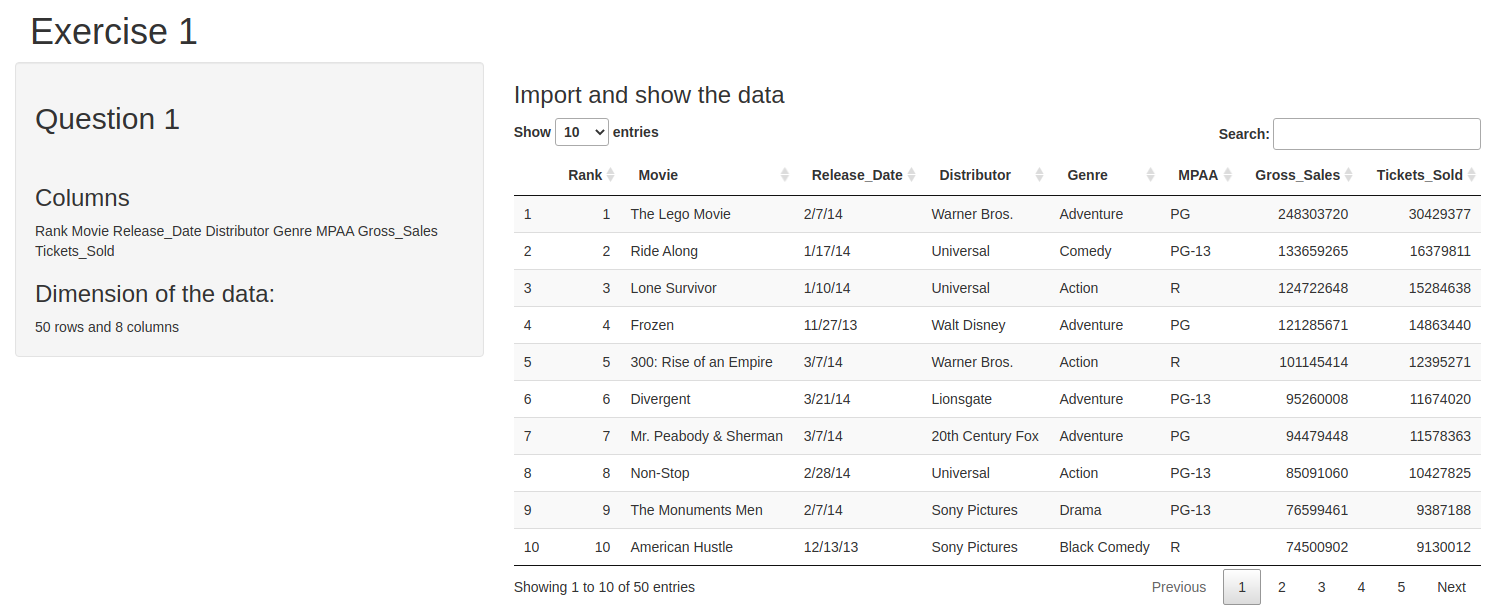
\includegraphics[width=\textwidth]{img/ex1_q1.png}
\end{frame}

\begin{frame}{Exercise 1 - Shiny (Movies dataset)}
    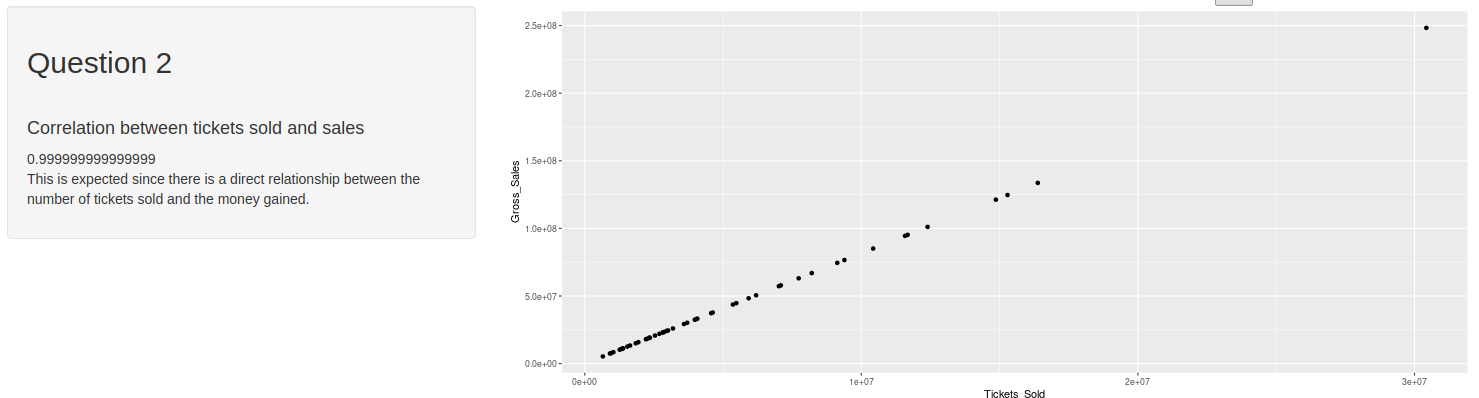
\includegraphics[width=\textwidth]{img/ex1_q2.png}
\end{frame}

\begin{frame}{Exercise 1 - Shiny (Movies dataset)}
    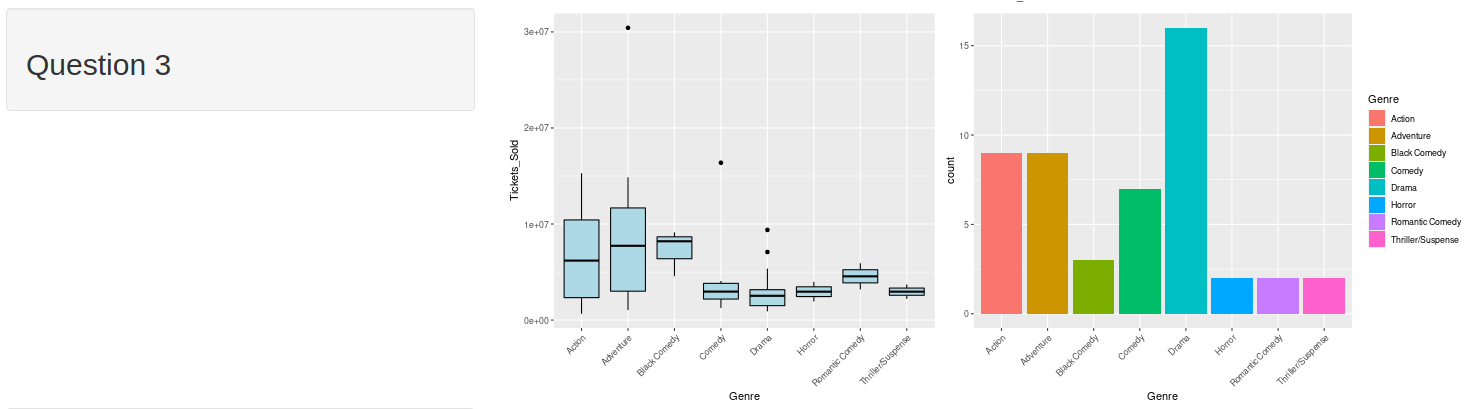
\includegraphics[width=\textwidth]{img/ex1_q3.png}
\end{frame}

\begin{frame}{Exercise 1 - Shiny (Movies dataset)}
    \movie[width=\textwidth, height=.8\textheight, loop]{Watch video}{img/R_exam_ex1_q3_animation.mp4}
    \href{https://youtu.be/NTgGG7UvRRU}{Backup link}: \footnotesize https://youtu.be/NTgGG7UvRRU
\end{frame}

\begin{frame}{Exercise 1 - Shiny (Movies dataset)}
    \movie[width=\textwidth, height=.8\textheight, loop]{Watch video}{img/R_exam_ex1_q4_animation.mp4}
    \href{https://youtu.be/w\_QQVsRoOpA}{Backup link}: \footnotesize https://youtu.be/w\_QQVsRoOpA
\end{frame}


\section{Exercise 2 - RMarkdown\\(Winter dataset)}
\begin{frame}{Exercise 1 - Shiny (Movies dataset)}
    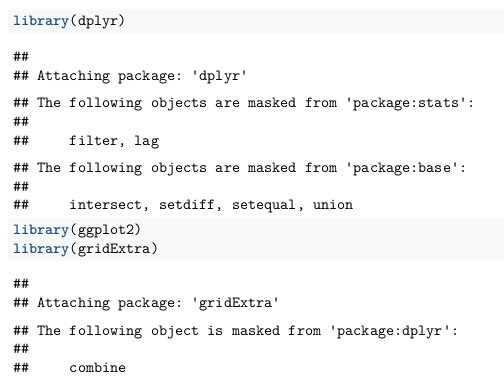
\includegraphics[width=\textwidth, height=\textheight]{img/ex2_part1_q1.png}
\end{frame}

\begin{frame}{Exercise 1 - Shiny (Movies dataset)}
    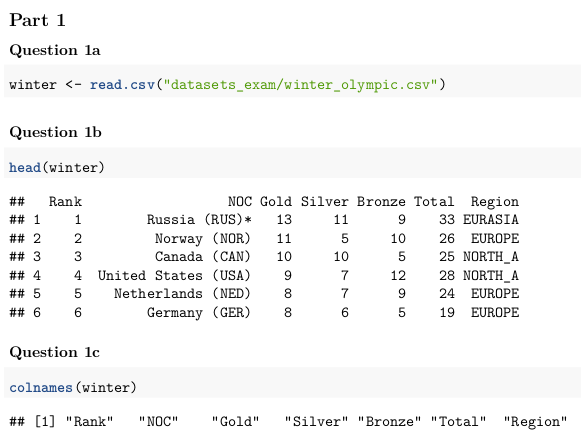
\includegraphics[width=\textwidth]{img/ex2_part1_q2.png}
\end{frame}

\begin{frame}{Exercise 1 - Shiny (Movies dataset)}
    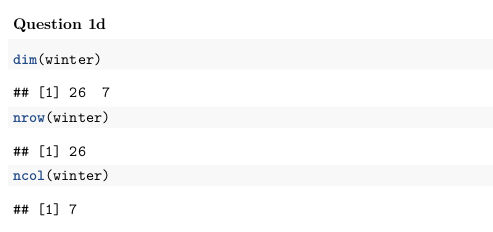
\includegraphics[width=\textwidth]{img/ex2_part1_q3.png}
\end{frame}



\section{Exercise 3 - Data Analysis\\(Summer-Winter dataset)}


\end{document}